\documentclass[../book.tex]{subfiles}
\graphicspath{{\subfix{../images/}}}

\begin{document}
\chapter{Inequalities}
\begin{introduction}[Contents]
\item Polynomial Inequalities
\item Rational Inequalities
\item Radical Inequalities
\item Exponential and Logarithmic Inequalities
\end{introduction}
\noindent The first half of this text covered the essential equation types, their properties, and how to graph them.  The goal of this chapter is to discuss the inequality versions of these equation types and to explore the similarities and differences between inequalities and equations.

Rather than combining these sections with their respective chapters, we chose to dedicate a specific chapter to them because we believed that it is best suited to learn them together.  Many of the methods seen in this chapter flow between sections, which would have been more difficult to convey between chapters.

We'll do these in the order of the previous chapters, starting with polynomial inequalities.
\section{Polynomial Inequalities}
\noindent This section will go over solving inequalities of any degree.  In order to solve these inequalities, we need to find the points in which the graph changes sign (usually at the roots of the polynomial).  We will use the examples to expand upon the method.

\begin{remark}
Note that we won't discuss linear inequalities in this section, since they are overly easy when compared to the difficulty of later problems.  If you can do those, linear problems will come much easier.
\end{remark}

\begin{example}
Find all $x$ such that $(x-2)(x-3)\geq 0$.
\end{example}
\begin{solution}
To solve a problem in factored form, we need to check every section of points.  In this case, there are the points such that $x\geq 3$, $2<x<3$, and $x\leq 2$.  In problems like these, we divide the regions by the intercepts since this is when the graph usually changes sign.

When $x\leq 2$, both $x-2$ and $x-3$ are non-positive (this is easiest seen by checking a point in the region, such as $x=0$).  Thus, $(x-2)(x-3)\geq 0$ when $x\leq 2$.  

When $2<x<3$, $x-2$ is positive but $x-3$ is negative (check $x=2.5$).  Thus, $(x-2)(x-3)<0$ when $2<x<3$.  

When $x\geq 3$, both $x-2$ and $x-3$ are non-negative.  Thus, $(x-2)(x-3)\geq 0$ when $x\geq 3$.  

This means we have two intervals that work.  We write these in interval notation, meaning the answer is $x\in(-\infty,2]\cup[3,\infty)$. $\Box$
\end{solution}
\begin{example}
Find all $x$ such that $2x^2+9x+4<0$.
\end{example}
\begin{solution}
We factor the quadratic to follow the same method as Example 14.1.  Factoring gives $(2x+1)(x+4)<0$.  Again, we split the function into three intervals: $x\leq-\dfrac{1}{2}$, $-\dfrac{1}{2}<x<4$, and $x\geq 4$.

When $x\leq -\dfrac{1}{2}$, this makes both the factors negative, leading to a positive product.  This is not what we want.

When $-\dfrac{1}{2}<x<4$, this makes the left factor negative and the right positive (check $x=0$), leading to a negative product.  This is what we are looking for, so we include this interval.

When $x>4$, this leads to two positive factors, giving a positive product.  Again, we don't want this.

We are left with one interval in the solution, which is $-\dfrac{1}{2}<x<4$. $\Box$
\end{solution}
\begin{example}
Find all $x$ such that $x^2-4x+2>0$.
\end{example}
\begin{solution}
We can quickly see that this quadratic does not factor.  Thus, we are forced to use the quadratic formula to solve this one.  We get $$x=\dfrac{4\pm\sqrt{16-4(1)(2)}}{2}=\dfrac{4\pm 2\sqrt{2}}{2}=2\pm\sqrt{2}.$$ Now we need to check the chunks, just like the previous problems.  Doing this finds the first and third intervals to be valid, just like Example 14.1.  Read the remark below to understand why.

The final interval of validity is $(-\infty,2-\sqrt{2})\cup(2+\sqrt{2},\infty)$. $\Box$
\end{solution}
\begin{remark}
The fact that the intervals are the same is not a coincidence.  Given a positive leading coefficient and a greater-than-sign, the first and last interval will always be correct.  This can be seen easily by graphing the quadratic.  If there is a less-than-sign, then the middle interval is the correct interval.  We will see this very soon when we discuss higher-order polynomials, because we will use this - along with the multiplicity - to more quickly find the valid intervals.
\end{remark}
Sometimes factoring isn't the best way to solve problems, since there are many instances when factoring isn't possible.  Rather than using the quadratic formula, let's consider a similar problem to Example 14.3 using the vertex form.  This also helps to see the answer when there are no real roots.
\begin{example}
Find all values of $x$ such that $y(x)=2x^2+8x+27$ is greater than zero.
\end{example}
\begin{solution}
If you attempt to use the quadratic formula, you find that there are no real roots (the discriminant is $-19$).  Instead, let's use vertex form.  This gives us $$y(x)=2(x^2+4x)+27=2(x+2)^2+27-8=2(x+2)^2+19.$$ We see that for all $x$, $(x+2)^2\geq 0$, meaning that $y(x)>0$ for all $x$.  So, our interval is $(-\infty,\infty)$. $\Box$
\end{solution}
We can also use this skill to find the range of various functions.  Let's use the next examples to find the range of a function.
\begin{example}
Let $f(x)=\dfrac{5x^2-4x+8}{x^2+1}$, where the domain of $f$ is $\mathbb{R}$.  Find the range of $f$.
\end{example}
\begin{solution}
Since every $x$-value must correspond to a $y$-value in the range of $f$, we need to find all values of $k$ such that $f(x)=k$.  Multiplying by $x^2+1$, and rearranging, we get $$(k-5)x^2+4x+(k-8)=0.$$ There must be at least one value of $x$ such that the discriminant of this polynomial is non-negative.  The discriminant of the polynomial is $$(4)^2-4(k-5)(k-8)\geq 0.$$  Solving this for $k$ by expanding gives us $$-k^2+13k-36\geq 0 \implies k^2-13k+36\leq 0 \implies k\in[4,9].$$  This means that $[4,9]$ is the range of $f$. $\Box$
\end{solution}
Now that we've discussed quadratic polynomials, let's discuss higher-order polynomials.  It is very much the same concept.  We will run through a few examples and discuss the common trend.
\begin{example}
Find all $x$ such that $x^3-7x+6>0$.
\end{example}
\begin{solution}
Similar to the quadratic problems discusses previously, we need to find the roots of the polynomial.  We've done this before in \hyperlink{chapter.6}{Chapter 6} when we discussed higher-order polynomials.  Using synthetic division, we find the roots.

Testing $x=1$ provides us a quick root.  Using synthetic division, we find that $$x^3-7x+6=(x-1)(x^2+x-6).$$  Factoring the quadratic, we get that $$x^3-7x+6=(x-1)(x+3)(x-2).$$  Plotting this on a number line, we get
\begin{figure}[!ht]
    \centering
    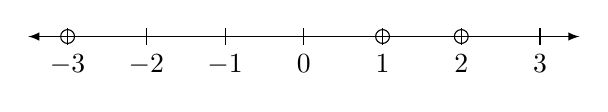
\begin{tikzpicture}
\draw[latex-latex] (-3.5,0) -- (3.5,0) ;
\foreach \x in  {-3,-2,-1,0,1,2,3}
\draw[shift={(\x,0)},color=black] (0pt,3pt) -- (0pt,-3pt);
\foreach \x in {-3,-2,-1,0,1,2,3}
\draw[shift={(\x,0)},color=black] (0pt,0pt) -- (0pt,-3pt) node[below] 
{$\x$};
\draw (1,0) circle[radius=2.5pt];
\draw (-3,0) circle[radius=2.5pt];
\draw (2,0) circle[radius=2.5pt];
\end{tikzpicture}
\end{figure}

We now need to check the areas around these points.  Checking $x=3$ (or an equivalent large number), all the factors are positive, so this region is valid.  Checking $x=1.5$, we get that the $(x-2)$ factor is negative, so the region is not valid.  Checking $x=0$, we get a positive number (it's easiest to check the un-factored form).  Checking $x=-4$ (or an equivalent small number), all factors are negative, so this region is not valid.

The filled-in number line is shown below.
\begin{figure}[!ht]
    \centering
    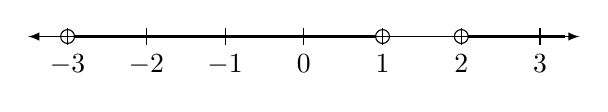
\begin{tikzpicture}
\draw[latex-latex] (-3.5,0) -- (3.5,0) ;
\foreach \x in  {-3,-2,-1,0,1,2,3}
\draw[shift={(\x,0)},color=black] (0pt,3pt) -- (0pt,-3pt);
\foreach \x in {-3,-2,-1,0,1,2,3}
\draw[shift={(\x,0)},color=black] (0pt,0pt) -- (0pt,-3pt) node[below] 
{$\x$};
\draw (1,0) circle[radius=2.5pt];
\draw (-3,0) circle[radius=2.5pt];
\draw (2,0) circle[radius=2.5pt];
\draw[very thick] (-2.92,0) -- (0.92,0);
\draw[very thick] (2.08,0) -- (3.32,0);
\end{tikzpicture}
\end{figure}

Reading the number line, we see the interval is $(-3,1)\cup(2,\infty)$. $\Box$
\end{solution}
You might notice that in all the examples we've covered that the intervals always alternate between positive and negative.  This is a great observation and is mostly true! There is one example when it isn't, which we see in the next example.
\begin{example}
Find all $x$ such that $x^3+2x^2-4x-8\leq 0$.
\end{example}
\begin{solution}
Hopefully you noticed to factor by grouping in this case.  Factoring this gets $$x^2(x+2)-4(x+2)=(x+2)(x^2-4)=(x+2)^2(x-2).$$  Drawing the number line, we get
\begin{figure}[!ht]
    \centering
    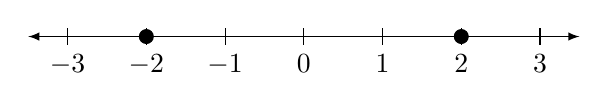
\begin{tikzpicture}
\draw[latex-latex] (-3.5,0) -- (3.5,0) ;
\foreach \x in  {-3,-2,-1,0,1,2,3}
\draw[shift={(\x,0)},color=black] (0pt,3pt) -- (0pt,-3pt);
\foreach \x in {-3,-2,-1,0,1,2,3}
\draw[shift={(\x,0)},color=black] (0pt,0pt) -- (0pt,-3pt) node[below] 
{$\x$};
\filldraw (-2,0) circle[radius=2.5pt];
\filldraw (2,0) circle[radius=2.5pt];
\end{tikzpicture}
\end{figure}

When we check values of $x$, note that $(x+2)^2$ is always positive.  This means we only have to check the $(x-2)$ factor.  If we check the rightmost interval ($x=3$ works), we get a positive value, which is invalid.  Checking $x=0$ (the middle interval), this is a negative value, which is valid.  Checking $x=-3$ (the leftmost interval), we get a negative value.

The filled in number line is shown below.
\begin{figure}[!ht]
    \centering
    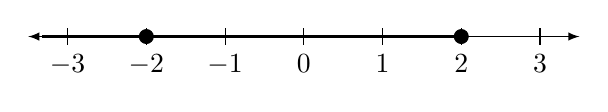
\begin{tikzpicture}
\draw[latex-latex] (-3.5,0) -- (3.5,0) ;
\foreach \x in  {-3,-2,-1,0,1,2,3}
\draw[shift={(\x,0)},color=black] (0pt,3pt) -- (0pt,-3pt);
\foreach \x in {-3,-2,-1,0,1,2,3}
\draw[shift={(\x,0)},color=black] (0pt,0pt) -- (0pt,-3pt) node[below] 
{$\x$};
\filldraw (-2,0) circle[radius=2.5pt];
\filldraw (2,0) circle[radius=2.5pt];
\draw[very thick] (-3.32,0) -- (1.92,0);
\end{tikzpicture}
\end{figure}

This leaves the interval $(-\infty,-2]\cup[-2,2]$, which can be simplified to $(-\infty,2]$. $\Box$
\end{solution}
This time it was different! We see that $-2$ has the same sign on both sides.  Why could this be?  Well, we know that $-2$ in this case has a multiplicity of $2$, meaning that graphically the function remains on the same side of the axis.  Look at the theorem below to see the formal definition.
\begin{theorem}{Multiplicity Rules for Inequalities}{mri}
Given a function $f(x)$ that can be factored into $$f(x)=k(x-x_1)^{a_1}(x-x_2)^{a_2}\ldots(x-x_n)^{a_n}$$ for some real constants $x_1$,$x_2$,$\ldots$,$x_n$, positive constants $a_1$,$a_2$,$\ldots$,$a_n$, and non-zero $k\in\mathbb{R}$, we determine the behavior of factor $(x-x_i)^{a_i}$ (where $i\leq n$) as follows: \begin{itemize}
    \item If $a_i$ is even, then $x_i$ will have the same sign on both sides of $x_i$.
    \item If $a_i$ is odd, then $x_i$ will switch signs going across $x_i$.
\end{itemize}
We use this rule to quickly determine the "sign chart" for the function.
\end{theorem}
Let's attempt to use this theorem in action in a fourth-degree problem.
\begin{example}
Find all $x$ such that $x^4-4x^3-3x^2+14x-8>0$.
\end{example}
\begin{solution}
We need to factor this, and it might take a few tries to do.  Quickly checking $x=1$, we realize that it works.  This gives us $$x^4-4x^3-3x^2+14x-8=(x-1)(x^3-3x^2-6x+8).$$ We check $x=1$ again and it works again!  This gives us $$x^4-4x^3-3x^2+14x-8=(x-1)^2(x^2-2x-8).$$ Factoring this, we get $$x^4-4x^3-3x^2+14x-8=(x-1)^2(x+2)(x-4).$$  Now, we can use Theorem 15.1 to our advantage.  The number line shows us 
\begin{figure}[!ht]
    \centering
    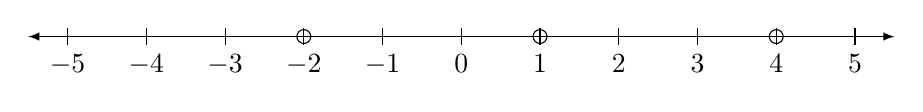
\begin{tikzpicture}
\draw[latex-latex] (-5.5,0) -- (5.5,0) ;
\foreach \x in  {-5,-4,-3,-2,-1,0,1,2,3,4,5}
\draw[shift={(\x,0)},color=black] (0pt,3pt) -- (0pt,-3pt);
\foreach \x in {-5,-4,-3,-2,-1,0,1,2,3,4,5}
\draw[shift={(\x,0)},color=black] (0pt,0pt) -- (0pt,-3pt) node[below] 
{$\x$};
\draw (1,0) circle[radius=2.5pt];
\draw (-2,0) circle[radius=2.5pt];
\draw (4,0) circle[radius=2.5pt];
\end{tikzpicture}
\end{figure}

We only need to check one value, and in this case it's easy to check a very high value.  This gives us a positive solution, which is valid.  Now, we follow the multiplicity rules.

$x=4$ has an odd multiplicity, so the sign changes to negative.  Then, the sign doesn't change around $x=1$.  Finally, it changes around $x=-2$.  

The filled-in number line looks like this:
\begin{figure}[!ht]
    \centering
    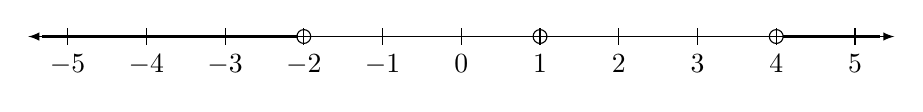
\begin{tikzpicture}
\draw[latex-latex] (-5.5,0) -- (5.5,0) ;
\foreach \x in  {-5,-4,-3,-2,-1,0,1,2,3,4,5}
\draw[shift={(\x,0)},color=black] (0pt,3pt) -- (0pt,-3pt);
\foreach \x in {-5,-4,-3,-2,-1,0,1,2,3,4,5}
\draw[shift={(\x,0)},color=black] (0pt,0pt) -- (0pt,-3pt) node[below] 
{$\x$};
\draw (1,0) circle[radius=2.5pt];
\draw (-2,0) circle[radius=2.5pt];
\draw (4,0) circle[radius=2.5pt];
\draw[very thick] (4.08,0) -- (5.32,0);
\draw[very thick] (-5.32,0) -- (-2.08,0);
\end{tikzpicture}
\end{figure}

Reading the number line, we see the interval is $(-\infty,-2)\cup(4,\infty)$. $\Box$
\end{solution}
Now, let's use this knowledge and expand to rational functions.  This won't be much more difficult than these examples; there's just one more step.
\section{Rational Inequalities}
\noindent Rational Inequalities follow a similar process to the one seen in the \hyperlink{section.14.2}{previous} section.  However, we must account for one more factor not seen in polynomials: discontinuities. Again, we will be solving functions such that $f(x)<0$, $f(x)>0$, $f(x)\leq 0$, and $f(x)\geq 0$.

First, the rational functions must be combined into a single fraction; however, expansion of polynomials is discouraged.  It is best to factor all denominators (and leave them factored) throughout this process.  Then, once one fraction is achieved; take note of all discontinuities (removable or non-removable).  These will be marked on the number line as open-holes.  Finally, find the roots of the numerator using the same method as before.  In short, we are using the methods outlined in \hyperlink{chapter.7}{Chapter 7} to locate the zeroes and the discontinuities, then "checking the chunks" as we did with polynomials.
\begin{example}
Find all values of $x$ such that $\dfrac{x^3-15x^2+74x-120}{x^2-8x+12}\leq 0$.  Write your answer in interval notation.
\end{example}
\begin{solution}
First, we need to factor the fraction to find the roots of both polynomials. The denominator is easy; we see that $x^2-8x+12=(x-2)(x-6)$. Factoring the numerator is a bit harder.  Checking small values for $x$ don't work.  Trying $x=5$ works (there's a reason for choosing this first, but it's beyond the scope of this book).  Synthetic division gives us:

\polyhornerscheme[x=5]{x^3-15x^2+74x-120}

This leaves us with $x^3-15x^2+74x-120=(x-5)(x^2-10x+24)$.  Factoring the quadratic gives us $x^3-15x^2+74x-120=(x-5)(x-4)(x-6)$.  Let's rewrite the original problem in factored form.  $$\dfrac{x^3-15x^2+74x-120}{x^2-8x+12}\leq 0 \implies \dfrac{(x-4)(x-5)(x-6)}{(x-2)(x-6)}\leq 0.$$ We notice that there's a removable discontinuity at $x=6$ and a non-removable discontinuity at $x=2$.  Although they are different, we need to account for both of them. We make this different since it will help with an advanced trick demonstrated at the end of the section. 

Let's make a number line with the roots and the discontinuities.
\begin{figure}[!ht]
    \centering
    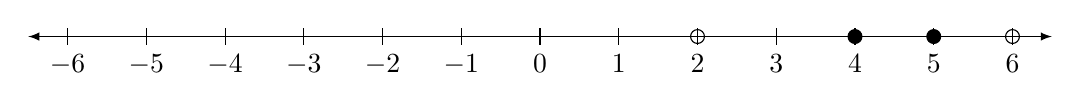
\begin{tikzpicture}
\draw[latex-latex] (-6.5,0) -- (6.5,0) ;
\foreach \x in  {-6,-5,-4,-3,-2,-1,0,1,2,3,4,5,6}
\draw[shift={(\x,0)},color=black] (0pt,3pt) -- (0pt,-3pt);
\foreach \x in {-6,-5,-4,-3,-2,-1,0,1,2,3,4,5,6}
\draw[shift={(\x,0)},color=black] (0pt,0pt) -- (0pt,-3pt) node[below] 
{$\x$};
\draw (2,0) circle[radius=2.5pt];
\draw (6,0) circle[radius=2.5pt];
\filldraw (4,0) circle[radius=2.5pt];
\filldraw (5,0) circle[radius=2.5pt];
\end{tikzpicture}
\end{figure}

Now, we can check the intervals. For these, it is easiest to look at the signs for each polynomial and use sign parity to determine the final sign.

At a large $x$, all terms are positive.  This leads to a positive value, which is not less than zero.  At $x=5.5$, the two negative terms are both $(x-6)$ terms, which cancel each other.  This still leads to a positive value, which is not less than zero.  At $x=4.5$, $(x-5)$ is also negative.  This leads to a negative value, which is less than zero.  At $x=3$, $(x-4)$ is now negative, cancelling the $(x-5)$ term.  The value is now positive, which is not less than zero.  At $x=0$, all terms are negative, leading to a negative product.  This is less than zero.

Plotting the filled-in number line, we get 
\begin{figure}[!ht]
    \centering
    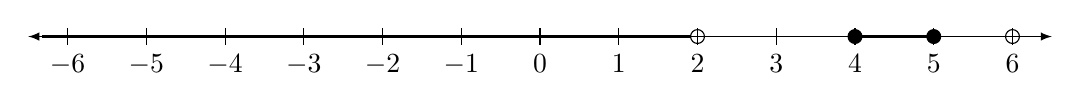
\begin{tikzpicture}
\draw[latex-latex] (-6.5,0) -- (6.5,0) ;
\foreach \x in  {-6,-5,-4,-3,-2,-1,0,1,2,3,4,5,6}
\draw[shift={(\x,0)},color=black] (0pt,3pt) -- (0pt,-3pt);
\foreach \x in {-6,-5,-4,-3,-2,-1,0,1,2,3,4,5,6}
\draw[shift={(\x,0)},color=black] (0pt,0pt) -- (0pt,-3pt) node[below] 
{$\x$};
\draw (2,0) circle[radius=2.5pt];
\draw (6,0) circle[radius=2.5pt];
\filldraw (4,0) circle[radius=2.5pt];
\filldraw (5,0) circle[radius=2.5pt];
\draw[very thick] (4.08,0) -- (4.92,0);
\draw[very thick] (-6.32,0) -- (1.92,0);
\end{tikzpicture}
\end{figure}

Reading the number line, we see that the final interval is $(-\infty,2)\cup[4,5]$. $\Box$
\end{solution}
This problem is going to escalate really quickly.  In doing this chapter, we believe that the ability to solve the hardest problem will make the simpler problems so much easier.  Let's look at the next example.
\begin{example}
Find all $x$ such that $\dfrac{x^3-10x^2+29x-20}{x^2-6x+9}\div\dfrac{x^2-6x}{x^3-12x^2+41x-30}\geq 0$.
\end{example}
\begin{solution}
This problem is much harder for a number of reasons.  Note the number of terms we have in division. We must keep track of all these discontinuities as we go.

First, we factor everything.  We quickly know that $x^2-6x=x(x-6)$ and $x^2-6x+9=(x-3)^2$.  Now, to factor the cubics.  Checking $x=1$ for $x^3-10x^2+29x-20$ works, and we get

\polyhornerscheme[x=1]{x^3-10x^2+29x-20}

\noindent Factoring the resultant polynomial gives us $x^2-9x+20=(x-4)(x-5)$; thus, $$x^3-10x^2+29x-20=(x-1)(x-4)(x-5).$$ Now for the other cubic.  Checking $x=1$ for $x^3-12x^2+41x-30$ works, and we get

\polyhornerscheme[x=1]{x^3-12x^2+41x-30}

\noindent Factoring the resultant polynomial gives us $x^2-11x-30=(x-5)(x-6)$, meaning that $$x^3-12x^2+41x-30=(x-1)(x-5)(x-6).$$
We rewrite the problem in terms of these factored polynomials: $$\dfrac{(x-1)(x-4)(x-5)}{(x-3)^2}\div\dfrac{x(x-6)}{(x-1)(x-5)(x-6)}\geq 0.$$
Now we need to note all the discontinuities here.  We easily tell that $x=3$ is a discontinuity as well as $x=1$, $x=5$, and $x=6$.  Are there any more? There is! Since the entire second term is divided, we need to find when the entire term equals zero, which is when $x=0$ and $x=6$. Compiling the numbers, we have discontinuities at $x=0,1,3,5,6$.

Now, when is $x$ valid? It's when the numerator of the first fraction equals zero, which is when $x=1,4,5$. The two discrepancies are at $x=1,5$, meaning $x$ is valid only at $x=4$.

Let's check to see if any are removable.  We flip the second fraction and multiply to get $$\dfrac{(x-1)(x-4)(x-5)}{(x-3)^2}\cdot\dfrac{(x-1)(x-5)(x-6)}{x(x-6)}\geq 0.$$ The only term that cancels is $x=6$, meaning it's the only removable discontinuity. Let's get to plotting.

\begin{figure}[!ht]
    \centering
    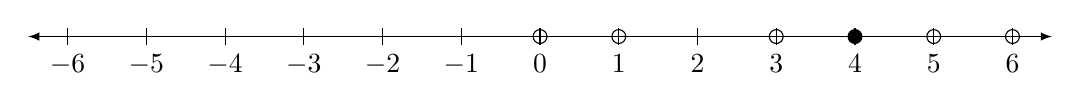
\begin{tikzpicture}
\draw[latex-latex] (-6.5,0) -- (6.5,0) ;
\foreach \x in  {-6,-5,-4,-3,-2,-1,0,1,2,3,4,5,6}
\draw[shift={(\x,0)},color=black] (0pt,3pt) -- (0pt,-3pt);
\foreach \x in {-6,-5,-4,-3,-2,-1,0,1,2,3,4,5,6}
\draw[shift={(\x,0)},color=black] (0pt,0pt) -- (0pt,-3pt) node[below] 
{$\x$};
\draw (0,0) circle[radius=2.5pt];
\draw (1,0) circle[radius=2.5pt];
\draw (3,0) circle[radius=2.5pt];
\draw (5,0) circle[radius=2.5pt];
\draw (6,0) circle[radius=2.5pt];
\filldraw (4,0) circle[radius=2.5pt];
\end{tikzpicture}
\end{figure}

Let's start checking.  There are six factors that need checking (since $(x-6)$ always cancels itself and $(x-3)^2$ is always positive).  However, we must check all chunks.

At large $x$, all factors are positive, which leads to a positive product.  At $x=5.5$, $(x-6)$ all important factors are still positive, leading to a positive product.  At $x=4.5$, $(x-5)$ turns negative, giving a negative product.  At $x=3.5$, both $(x-4)$ and $(x-5)$ are negative, leading to a positive product.  At $x=2$, the important factors have the same sign, again leading to a positive product.  At $x=0.5$, $(x-1)$ turns negative, leading to a negative product.  At $x=-1$, all factors are negative, leading to a positive product.

Below is the filled-in number line containing this data.

\begin{figure}[!ht]
    \centering
    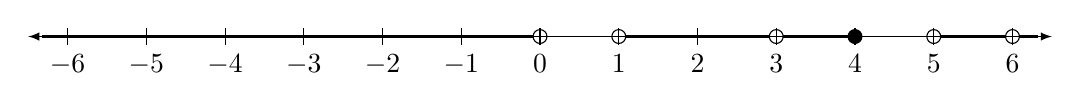
\begin{tikzpicture}
\draw[latex-latex] (-6.5,0) -- (6.5,0) ;
\foreach \x in  {-6,-5,-4,-3,-2,-1,0,1,2,3,4,5,6}
\draw[shift={(\x,0)},color=black] (0pt,3pt) -- (0pt,-3pt);
\foreach \x in {-6,-5,-4,-3,-2,-1,0,1,2,3,4,5,6}
\draw[shift={(\x,0)},color=black] (0pt,0pt) -- (0pt,-3pt) node[below] 
{$\x$};
\draw (0,0) circle[radius=2.5pt];
\draw (1,0) circle[radius=2.5pt];
\draw (3,0) circle[radius=2.5pt];
\draw (5,0) circle[radius=2.5pt];
\draw (6,0) circle[radius=2.5pt];
\filldraw (4,0) circle[radius=2.5pt];
\draw[very thick] (6.08,0) -- (6.32,0);
\draw[very thick] (5.08,0) -- (5.92,0);
\draw[very thick] (3.08,0) -- (3.92,0);
\draw[very thick] (1.08,0) -- (2.92,0);
\draw[very thick] (-6.32,0) -- (-0.08,0);
\end{tikzpicture}
\end{figure}

Writing this in interval notation gives us $(-\infty,0)\cup(1,3)\cup(3,4]\cup(5,6)\cup(6,\infty)$. $\Box$
\end{solution}

\noindent That is as hard as it's going to get.  In summary, for problems such as these, find all the discontinuities, then find the roots, then check the chunks.  Let's discuss a faster way to do this.

The last part of this section goes over a quick method to find the intervals.  This is an advanced method and is not for all viewers; don't be discouraged if you do not understand.  The method is an extension of the multiplicity rule mentioned in the \hyperlink{section.14.2}{previous} section to fit inequalities of all types.

\begin{wrapfigure}{r}{4cm}
    \begin{tikzpicture}[xscale=0.4,yscale=0.4]
      \draw[<->] (-5,0) -- (5,0) node[right] {$x$};
      \draw[<->] (0,-5) -- (0,5) node[above] {$y(x)$};
      \draw[domain=-5:1.92,smooth,variable=\x,blue] plot ({\x},{\x});
      \draw (2,2) circle[radius=2.5pt];
      \draw[domain=2.08:5,smooth,variable=\x,blue] plot ({\x},{\x});
    \end{tikzpicture}
\end{wrapfigure}

Theorem 15.1 gives us the rules for changing signs across a zero given a certain multiplicity; however, it only works for non-removable discontinuities.  We must note that removable discontinuities do not abide by this.  Since removable discontinuities are holes $-$ rather than asymptotes $-$ the graph won't change sign since the graph doesn't move.

Consider the graph to the right of $f(x)=\dfrac{x(x-2)}{x-2}$.  We see that there is a hole at $x=2$, but the graph doesn't change signs. This is because the hole doesn't move the graph, it just impacts the domain (and the range) by a single value.

We summarize the multiplicity extension in Theorem 15.2 to determine whether we change signs or not.
\begin{theorem}{Extension of the Multiplicity Rule}{extmult}
Given a rational function $f(x)$ that has denominator $$k(x-x_1)^{a_1}(x-x_2)^{a_2}\ldots(x-x_n)^{a_n}$$ for some real constants $x_1$,$x_2$,$\ldots$,$x_n$, positive constants $a_1$,$a_2$,$\ldots$,$a_n$, and non-zero $k\in\mathbb{R}$, we determine the behavior of factor $(x-x_i)^{a_i}$ (where $i\leq n$) as follows: \begin{itemize}
    \item If $a_i$ is even, then $x_i$ will have the same sign on both sides of $x_i$.
    \item If $a_i$ is odd, then $x_i$ will switch signs going across $x_i$.
    \item If $x_i$ is a removable discontinuity, $x_i$ will have the same sign on both sides of $x_i$.
\end{itemize}
Adding this third rule will allow us to use this rule for rational inequalities as well.
\end{theorem}
Let's try one last example where we use Theorem 15.2 to make this process easier.
\begin{example}
Find all values of $x$ such that $\dfrac{x^2-16}{x^2+5x+6} \div \dfrac{x^2+5x+4}{x^2-2x-8} \leq 0.$
\end{example}
\begin{solution}
The first step is to factor all the polynomials.  They are all easily factorable and are not the major point of this example.  We won't show the work factoring these $-$ here is the example written in factored form:
$$\dfrac{(x+4)(x-4)}{(x+2)(x+3)}\div\dfrac{(x+1)(x+4)}{(x-4)(x+2)}\leq 0.$$
We note all the discontinuities as $x=-3,-2$ from the first denominator, $x=-4,-1$ from the second numerator, and $x=-2,4$ from the second denominator.  We flip the second fraction: $$\dfrac{(x+4)(x-4)}{(x+2)(x+3)}\cdot\dfrac{(x-4)(x+2)}{(x+1)(x+4)}\leq 0 \implies \dfrac{(x-4)^2}{(x+1)(x+3)}\leq 0.$$
From this, we can see that $(x+2)$ and $(x+4)$ both cancel, so $x=-4,-2$ are removable, while $x=-3,-1,4$ are all non-removable.

Finding the roots, we get $x=-4,4$.  These both conflict with the discontinuities, meaning that there are no roots.

Let's plot the number line.

\begin{figure}[!ht]
    \centering
    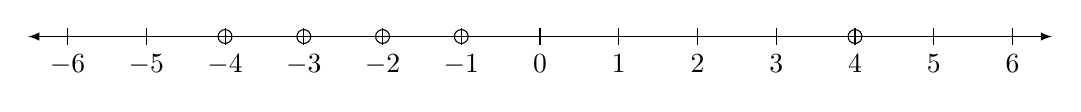
\begin{tikzpicture}
\draw[latex-latex] (-6.5,0) -- (6.5,0) ;
\foreach \x in  {-6,-5,-4,-3,-2,-1,0,1,2,3,4,5,6}
\draw[shift={(\x,0)},color=black] (0pt,3pt) -- (0pt,-3pt);
\foreach \x in {-6,-5,-4,-3,-2,-1,0,1,2,3,4,5,6}
\draw[shift={(\x,0)},color=black] (0pt,0pt) -- (0pt,-3pt) node[below] 
{$\x$};
\draw (-4,0) circle[radius=2.5pt];
\draw (-3,0) circle[radius=2.5pt];
\draw (-2,0) circle[radius=2.5pt];
\draw (-1,0) circle[radius=2.5pt];
\draw (4,0) circle[radius=2.5pt];
\end{tikzpicture}
\end{figure}

Now, let's try to use the multiplicity rules.  We check a very large $x$ and see the value is positive.  Now, let's use the multiplicity rules to guide us.

$x=4$ is a squared term, meaning that we don't change sign, meaning it's still positive.  $x=-1$ is a non-removable, linear term, so we change sign, meaning it's now negative. At $x=-2$, we have a removable discontinuity, so we don't change sign, meaning it's still negative.  At $x=-3$, we have a non-removable, linear discontinuity, so we change the sign, meaning it's now positive.  At $x=-4$, we have a removable discontinuity, meaning we don't change sign, so it's still positive.

Let's take a look at the filled-in number line.

\begin{figure}[!ht]
    \centering
    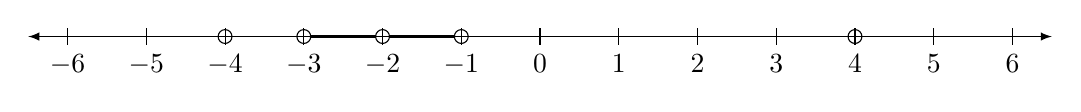
\begin{tikzpicture}
\draw[latex-latex] (-6.5,0) -- (6.5,0) ;
\foreach \x in  {-6,-5,-4,-3,-2,-1,0,1,2,3,4,5,6}
\draw[shift={(\x,0)},color=black] (0pt,3pt) -- (0pt,-3pt);
\foreach \x in {-6,-5,-4,-3,-2,-1,0,1,2,3,4,5,6}
\draw[shift={(\x,0)},color=black] (0pt,0pt) -- (0pt,-3pt) node[below] 
{$\x$};
\draw (-4,0) circle[radius=2.5pt];
\draw (-3,0) circle[radius=2.5pt];
\draw (-2,0) circle[radius=2.5pt];
\draw (-1,0) circle[radius=2.5pt];
\draw (4,0) circle[radius=2.5pt];
\draw[very thick] (-2.92,0) -- (-2.08,0);
\draw[very thick] (-1.92,0) -- (-1.08,0);
\end{tikzpicture}
\end{figure}
Looking at the interval, the values of $x$ we need are at $(-3,-2)\cup(-2,-1)$. $\Box$
\end{solution}
Congrats! You got through the hardest example.  Hopefully the method made a bit of sense; it takes some practice to understand and implement, but once you get it, it's very rewarding.

This was the hardest section of the chapter, so it's downhill from here.  We move on to radical inequalities next.
\section{Radical Inequalities}
\noindent The goal in this section is to extend the ideas from \hyperlink{chapter.8}{Chapter 8} by adding inequalities.  This time, unlike the previous sections, we can use inequalities for approximation of square roots.  Since we don't have a great method for evaluating the value of a square root, we can use approximation techniques with inequalities instead.

Let's begin with an easier example.
\begin{example}
Find all real $x$ such that $3\sqrt{x}\geq x+2$.
\end{example}
\begin{solution}
We first note that for $\sqrt{x}$ to be defined, we must have $x\geq 0$, which means that $x+2\geq 0$. These are both true, so we look for any restrictions in the whole inequality.

Squaring both sides, we get $9x\geq x^2+4x+4$.  Rearranging gives us $x^2-5x+4\leq 0$, which gives us $(x-1)(x-4)\leq 0$.  This is only true when $x\in[1,4]$. $\Box$
\end{solution}
We still need to be really careful when we square both sides, possibly even more careful.  Be sure that you don't flip the equation and not change the direction of the inequality.  Also, as seen in the previous example, we ensured that both sides weren't negative before squaring. What might happen if you don't? Let's find out.
\begin{example}
Find all $x$ such that $\sqrt{x+2}\leq -x$.
\end{example}
\begin{solution}
We quickly notice that $x\geq -2$ in order for the left side to be defined.  The right side seems tricky, and we can't quite square both sides without noting an exception.  We can easily see by plugging in numbers that all positive $x$ are valid here, but there may be some negative value of $x$ where this isn't valid.  This means that we only consider the interval from $[-2,0]$ when we square both sides.

When we do this, we get $x+x\geq x^2$. Rearranging gives us $x^2-x-2\leq 0$, meaning that $(x-2)(x+1)\leq 0$.  This means that the interval $[-1,2]$ is valid.  Combining this with the $[0,\infty)$ interval, we get the final interval of $[-1,\infty)$. $\Box$
\end{solution}
Be sure you understand what we did here.  At first, it does not make much sense, because it contradicts checking to make sure both sides are non-negative.  Squaring both sides is a dangerous maneuver, so this is a perfect example of why we need to be conscious of possible mistakes we might make.

Let's move on to attempt a problem with a cube root. Surprisingly, it's actually easier!
\begin{example}
Find all $x$ such that $\sqrt[3]{2x^2+3x-26}<x-2$.
\end{example}
\begin{solution}
This time, we will cube to get rid of cube roots.  What happened to checking both sides to make sure that they're positive?  We don't have to do that this time!  The domain and range of cube root functions are $\mathbb{R}$, so there are no restrictions to worry about.

Cubing both sides gives us $2x^2+3x-26=(x-2)^3$.  Expand $(x-2)^3$ using a method of your choice to get $$2x^2+3x-26=x^3-6x^2+12x-8.$$ We move all the terms to one side and get $x^3-8x^2+9x+18=0$ and factor.  This gives us $(x+1)(x-3)(x-6)=0$, meaning that $x=-1,3,6$. Now, we can check the chunks.

Drawing the number line gives us:

\begin{figure}[!ht]
    \centering
    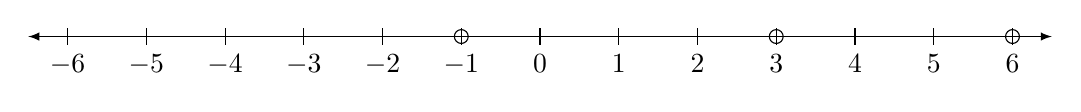
\begin{tikzpicture}
\draw[latex-latex] (-6.5,0) -- (6.5,0) ;
\foreach \x in  {-6,-5,-4,-3,-2,-1,0,1,2,3,4,5,6}
\draw[shift={(\x,0)},color=black] (0pt,3pt) -- (0pt,-3pt);
\foreach \x in {-6,-5,-4,-3,-2,-1,0,1,2,3,4,5,6}
\draw[shift={(\x,0)},color=black] (0pt,0pt) -- (0pt,-3pt) node[below] 
{$\x$};
\draw (-1,0) circle[radius=2.5pt];
\draw (3,0) circle[radius=2.5pt];
\draw (6,0) circle[radius=2.5pt];
\end{tikzpicture}
\end{figure}

We can check the chunks using the polynomial rather than the radical since they are indeed the same function.  We use the multiplicity extension to solve this; if you aren't comfortable with this method, use the method you are most comfortable using.

Applying this method fills in the number line as follows:

\begin{figure}[!ht]
    \centering
    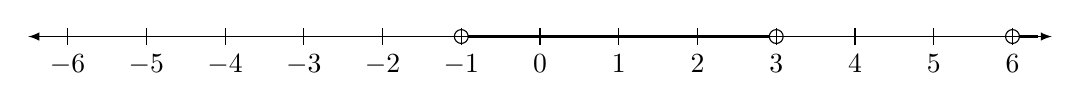
\begin{tikzpicture}
\draw[latex-latex] (-6.5,0) -- (6.5,0) ;
\foreach \x in  {-6,-5,-4,-3,-2,-1,0,1,2,3,4,5,6}
\draw[shift={(\x,0)},color=black] (0pt,3pt) -- (0pt,-3pt);
\foreach \x in {-6,-5,-4,-3,-2,-1,0,1,2,3,4,5,6}
\draw[shift={(\x,0)},color=black] (0pt,0pt) -- (0pt,-3pt) node[below] 
{$\x$};
\draw (-1,0) circle[radius=2.5pt];
\draw (3,0) circle[radius=2.5pt];
\draw (6,0) circle[radius=2.5pt];
\draw[very thick] (-0.92,0) -- (2.92,0);
\draw[very thick] (6.08,0) -- (6.32,0);
\end{tikzpicture}
\end{figure}
Writing this in interval notation, we get $(-1,3)\cup(6,\infty)$. $\Box$
\end{solution}
We still don't have a great method for approximating square root functions unless the argument is a perfect square.  Let's see if inequalities can help.
\begin{example}
Find the smallest $x$ such that $\sqrt{x}-\sqrt{x-1}<0.01$.
\end{example}
\begin{solution}
Now that we have two radical functions, we have even less of an idea of how to approximate it $-$ even for a perfect square.  However, we may be able to estimate $\sqrt{x}+\sqrt{x-1}$ a bit easier if $x$ is a perfect square.  We multiply by this value on both sides to get $$1<\dfrac{1}{100}(\sqrt{x}+\sqrt{x-1}) \implies 100<\sqrt{x}+\sqrt{x-1}.$$
We can find a value for this pretty quickly.  Since $\sqrt{x}\approx\sqrt{x-1}$ for a large $x$, we can look for values of $x$ such that both terms are approximately $50$.  Let $x=50^2$. This means that $\sqrt{x}=50$ and $\sqrt{x-1}<50$, so $\sqrt{x}+\sqrt{x-1}<100$. Letting $x=50^2+1$, we get $\sqrt{x}>50$ and $\sqrt{x-1}=50$, meaning $\sqrt{x}+\sqrt{x-1}>100$.

Therefore, the smallest value of $x$ that satisfies the inequality is $x=50^2+1=2501.$ $\Box$
\end{solution}
This section was pretty short when compared to the other sections; however, radical inequalities aren't much different than radical equations.

Next, we cover the final type of function and how to deal with their inequalities: exponential and logarithmic functions.
\section{Exponential and Logarithmic Inequalities}
\noindent Exponential and Logarithmic Inequalities are the final types of inequalities discussed in this chapter.  They combine elements seen in the previous sections (primarily radical inequalities), meaning there isn't much new information to be covered.

This section will be among the shortest in the chapter, but it is important that we cover this information.
\begin{example}
Find all values of $x$ that satisfy $\log_{10}(x-12)\leq 2$.
\end{example}
\begin{solution}
First, we need to note any domain restrictions on the inequality.  We know that $\log(x-12)$ is only defined for $x>12$.  Raising both sides to the power of $10$, we get $x-12\leq 10^2$, meaning that $x\leq 112.$

However, because of the domain restriction, we must combine the intervals to get $(12,112]$. $\Box$
\end{solution}
Now that we understand how to account for domain restrictions, let's ramp up the difficulty to match other sections.
\begin{example}
Find the regions of all values of $x$ that satisfy $\log_2\left(\dfrac{(x-2)(x-4)}{(x-3)(x-5)^2}\right)\geq 0$. (A root-finder may be used for this problem.)
\end{example}
\begin{solution}
We again need to note domain restrictions here.  We see that $\dfrac{(x-2)(x-4)}{(x-3)(x-5)^2}> 0$, which is solvable using methods in the rational functions section.  We see the roots for the function are $x=2,4$ and the discontinuities are $x=3,5$.  Plotting the number line, we get 

\begin{figure}[!ht]
    \centering
    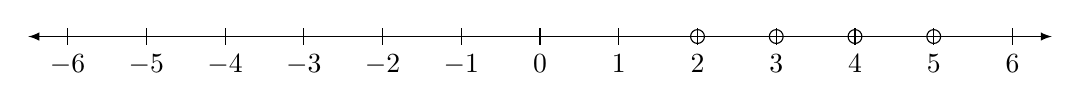
\begin{tikzpicture}
\draw[latex-latex] (-6.5,0) -- (6.5,0) ;
\foreach \x in  {-6,-5,-4,-3,-2,-1,0,1,2,3,4,5,6}
\draw[shift={(\x,0)},color=black] (0pt,3pt) -- (0pt,-3pt);
\foreach \x in {-6,-5,-4,-3,-2,-1,0,1,2,3,4,5,6}
\draw[shift={(\x,0)},color=black] (0pt,0pt) -- (0pt,-3pt) node[below] 
{$\x$};
\draw (2,0) circle[radius=2.5pt];
\draw (3,0) circle[radius=2.5pt];
\draw (4,0) circle[radius=2.5pt];
\draw (5,0) circle[radius=2.5pt];
\end{tikzpicture}
\end{figure}
\noindent Using the multiplicity rule, we can fill in the number line as follows:

\begin{figure}[!ht]
    \centering
    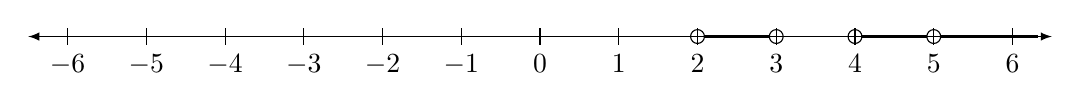
\begin{tikzpicture}
\draw[latex-latex] (-6.5,0) -- (6.5,0) ;
\foreach \x in  {-6,-5,-4,-3,-2,-1,0,1,2,3,4,5,6}
\draw[shift={(\x,0)},color=black] (0pt,3pt) -- (0pt,-3pt);
\foreach \x in {-6,-5,-4,-3,-2,-1,0,1,2,3,4,5,6}
\draw[shift={(\x,0)},color=black] (0pt,0pt) -- (0pt,-3pt) node[below] 
{$\x$};
\draw (2,0) circle[radius=2.5pt];
\draw (3,0) circle[radius=2.5pt];
\draw (4,0) circle[radius=2.5pt];
\draw (5,0) circle[radius=2.5pt];
\draw[very thick] (5.08,0) -- (6.32,0);
\draw[very thick] (4.08,0) -- (4.92,0);
\draw[very thick] (2.08,0) -- (2.92,0);
\end{tikzpicture}
\end{figure}
This shows us that the interval of validity here is $(2,3)\cup(4,5)\cup(5,\infty)$. Now, we need to find the interval for the entire problem.

Raising both sides to the power of $2$, we get $$\dfrac{(x-2)(x-4)}{(x-3)(x-5)^2}\geq 1 \implies (x-2)(x-4)>(x-3)(x-5)^2.$$ Expanding the polynomials and rearranging gives us $$x^2-6x+8\geq x^3-13x^2+55x-75 \implies x^3-14x^2+61x-83=0.$$ Here, we use the root-finder to find the roots as approximately $x=2.801, 4.287, 6.912$. We draw a number line for this data and get

\begin{figure}[!ht]
    \centering
    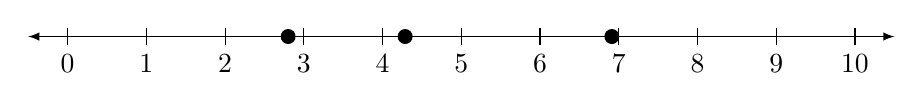
\begin{tikzpicture}
\draw[latex-latex] (-0.5,0) -- (10.5,0) ;
\foreach \x in  {0,1,2,3,4,5,6,7,8,9,10}
\draw[shift={(\x,0)},color=black] (0pt,3pt) -- (0pt,-3pt);
\foreach \x in {0,1,2,3,4,5,6,7,8,9,10}
\draw[shift={(\x,0)},color=black] (0pt,0pt) -- (0pt,-3pt) node[below] 
{$\x$};
\filldraw (2.801,0) circle[radius=2.5pt];
\filldraw (4.287,0) circle[radius=2.5pt];
\filldraw (6.912,0) circle[radius=2.5pt];
\end{tikzpicture}
\end{figure}

\noindent Using the multiplicity rule again, we can fill in the intervals as follows:

\begin{figure}[!ht]
    \centering
    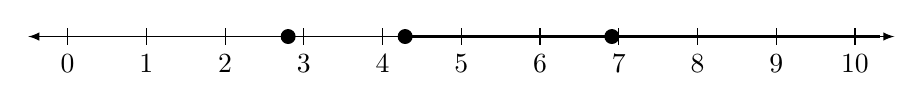
\begin{tikzpicture}
\draw[latex-latex] (-0.5,0) -- (10.5,0) ;
\foreach \x in  {0,1,2,3,4,5,6,7,8,9,10}
\draw[shift={(\x,0)},color=black] (0pt,3pt) -- (0pt,-3pt);
\foreach \x in {0,1,2,3,4,5,6,7,8,9,10}
\draw[shift={(\x,0)},color=black] (0pt,0pt) -- (0pt,-3pt) node[below] 
{$\x$};
\filldraw (2.801,0) circle[radius=2.5pt];
\filldraw (4.287,0) circle[radius=2.5pt];
\filldraw (6.912,0) circle[radius=2.5pt];
\draw[very thick] (6.992,0) -- (10.32,0);
\draw[very thick] (4.367,0) -- (6.832,0);
\end{tikzpicture}
\end{figure}

\noindent We now need to combine the intervals such that both are satisfied.  Doing this, we get the final interval of $[2.801]\cup[4.287,5)\cup(5,\infty).$ $\Box$
\end{solution}
These are about as hard as these problems are going to get.  All the practice problems, including the challenge problems, should not be difficult using the methods provided.  If something seems difficult, try a different method!
\begin{reviewset}
\item Find all $x$ that satisfy the inequalities below. \newline
(a) $6x^2+5x<4$. \hspace{\stretch{1}} (b) $x^2+50x-2079\geq 0$. \hspace{\stretch{1}} (c) $-x^2+7x-13>0$. \vspace{3mm}
\item Find all $x$ such that $\sqrt{x}<2x$. \vspace{3mm}
\item Let $f(x)=\dfrac{7x^2-4x+4}{x^2+1}$. Find the range of $f(x)$ given the domain of $f(x)$ to be all real numbers. \vspace{3mm}
\item Find the region of values of $x$ that satisfy the inequalities below. \newline 
(a) $\dfrac{x^2+x-6}{2x^3-9x^2+x+12}<0$. \hspace{\stretch{1}} (b) $\dfrac{x^2+x-2}{4x^2+11x-3}\div\dfrac{x^2+2x-3}{2x^2-9x-5}\geq 0.$ \vspace{3mm}
\item Solve the inequality $\sqrt{5x-1}+\sqrt{x-1}\leq 2$. \vspace{3mm}
\item Find the region of all $x$ that satisfies $\log\left(\dfrac{x^2-4}{x-4}\right)\geq 3$. \vspace{2mm}
\item Solve the following inequalities: \newline 
(a) $\log_5(3-x)\geq 7$ \hspace{50mm} (b) $\log_{(1/2)}(2x)>3$. \vspace{3mm}
\item Find all $x$ such that $\sqrt[3]{5x^2+24x+8}-2<x$. \vspace{3mm}
\item To the nearest thousandth, $\log_{10}(2)=0.301$ and $\log_{10}(3)=0.477$. Which of the following is the best approximation of $\log_5(10)$? \newline 
$$\dfrac{8}{7},\hspace{8mm}\dfrac{9}{7},\hspace{8mm}\dfrac{10}{7},\hspace{8mm}\dfrac{11}{7},\hspace{8mm}\dfrac{12}{7}.$$ \vspace{3mm}
\item Let $x>0$ and $y\leq c$ where $c$ is a constant.  Prove that $\dfrac{x+y}{1+\dfrac{xy}{c^2}}\leq c$. \vspace{3mm}
\item Below is the number line indicating a solution for some polynomial function $f(x)$.  Using this, determine the original function.
\begin{figure}[!ht]
    \centering
    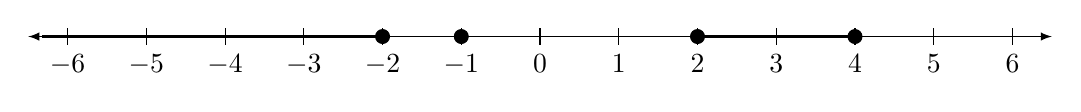
\begin{tikzpicture}
\draw[latex-latex] (-6.5,0) -- (6.5,0) ;
\foreach \x in  {-6,-5,-4,-3,-2,-1,0,1,2,3,4,5,6}
\draw[shift={(\x,0)},color=black] (0pt,3pt) -- (0pt,-3pt);
\foreach \x in {-6,-5,-4,-3,-2,-1,0,1,2,3,4,5,6}
\draw[shift={(\x,0)},color=black] (0pt,0pt) -- (0pt,-3pt) node[below] 
{$\x$};
\filldraw (-2,0) circle[radius=2.5pt];
\filldraw (-1,0) circle[radius=2.5pt];
\filldraw (2,0) circle[radius=2.5pt];
\filldraw (4,0) circle[radius=2.5pt];
\draw[very thick] (-6.32,0) -- (-2.08,0);
\draw[very thick] (2.08,0) -- (3.92,0);
\end{tikzpicture}
\end{figure} \vspace{3mm}

\item Without using a calculator, determine which is greater: $\dfrac{445721}{9902923}$ or $\dfrac{445725}{9902927}$. \vspace{3mm}
\end{reviewset}
\begin{challengeset}
\item Find all values of $x$ such that $\sqrt{x^2+7x+10}>x+2+\sqrt{x+2}$. \vspace{3mm}
\item Let $a\geq b>1$. What is the largest possible value of $\log_a{\left(\dfrac{a}{b}\right)}+\log_b{\left(\dfrac{b}{a}\right)}$? \vspace{3mm}
\item If $\log_2(a)+\log_2(b)\geq 6$, then find the smallest possible value of $a+b$. \vspace{3mm}
\item If $x,y>0$, $\log_y(x)+\log_x(y)=\dfrac{10}{3}$, and $xy=144$, find the value of $\dfrac{x+y}{2}$. \vspace{2mm}
\item Prove that $\dfrac{x^2+2}{\sqrt{x^2+1}}\geq 2$. \vspace{3mm}
\item Below is the number line indicating a solution for some rational function $f(x)$.  Given that no discontinuities are removable, determine the original function.
\begin{figure}[!ht]
    \centering
    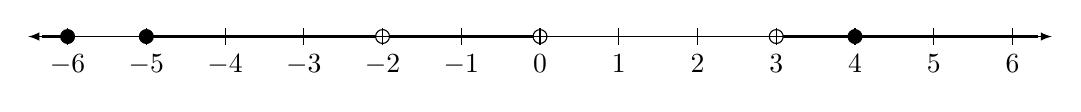
\begin{tikzpicture}
\draw[latex-latex] (-6.5,0) -- (6.5,0) ;
\foreach \x in  {-6,-5,-4,-3,-2,-1,0,1,2,3,4,5,6}
\draw[shift={(\x,0)},color=black] (0pt,3pt) -- (0pt,-3pt);
\foreach \x in {-6,-5,-4,-3,-2,-1,0,1,2,3,4,5,6}
\draw[shift={(\x,0)},color=black] (0pt,0pt) -- (0pt,-3pt) node[below] 
{$\x$};
\filldraw (-6,0) circle[radius=2.5pt];
\filldraw (-5,0) circle[radius=2.5pt];
\filldraw (4,0) circle[radius=2.5pt];
\draw (-2,0) circle[radius=2.5pt];
\draw (3,0) circle[radius=2.5pt];
\draw (0,0) circle[radius=2.5pt];
\draw[very thick] (-6.32,0) -- (-6.08,0);
\draw[very thick] (-4.92,0) -- (-2.08,0);
\draw[very thick] (-1.92,0) -- (-0.08,0);
\draw[very thick] (3.08,0) -- (3.92,0);
\draw[very thick] (4.08,0) -- (6.32,0);
\end{tikzpicture}
\end{figure} \vspace{3mm}
\item Using the function found from the previous problem, determine a two-dimensional graph that graphs the function and the solution intervals. \vspace{3mm}
\item Show that $\dfrac{1}{10}<\sqrt{101}-\sqrt{99}$ without using a calculator. \vspace{3mm}
\item Find all $x$ such that $\left(x^2-x-1\right)^{\left(x^2+x-20\right)}<1$. \vspace{3mm}
\item Find the largest integer $n$ such that $n<\left(\sqrt{33+\sqrt{128}}+\sqrt{2}-8\right)^{-1}$. \vspace{3mm}
\end{challengeset}
\end{document}